\documentclass[tikz,border=2mm]{standalone}

\usetikzlibrary{
  arrows.meta,
  calc,
  shapes.geometric
}

\begin{document}

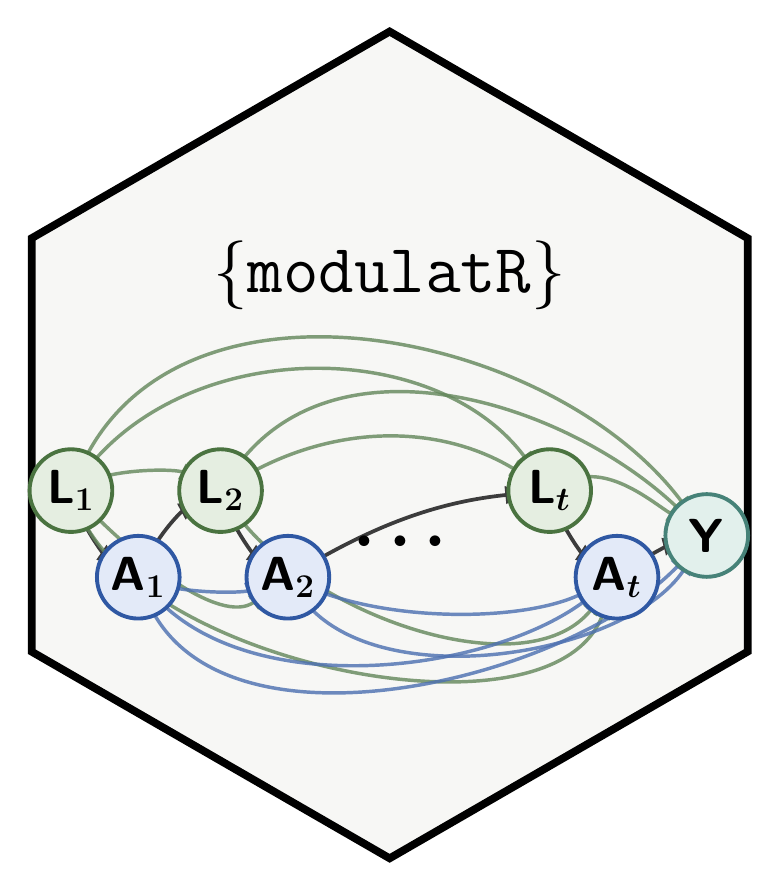
\begin{tikzpicture}[>=Latex]

% --------------------------------------------------
% Colors
% --------------------------------------------------
\definecolor{hexbg}{RGB}{247,247,245}

\definecolor{Ldraw}{RGB}{74,115,64}
\definecolor{Lfill}{RGB}{229,238,225}

\definecolor{Adraw}{RGB}{47,88,163}
\definecolor{Afill}{RGB}{227,234,248}

\definecolor{Ydraw}{RGB}{70,130,120}
\definecolor{Yfill}{RGB}{226,240,236}

\definecolor{mainarrow}{RGB}{60,60,60}

% --------------------------------------------------
% Styles
% --------------------------------------------------
\tikzset{
  baseNode/.style={
    circle,
    line width=1.4pt,
    minimum size=10.5mm,
    inner sep=0pt,
    font=\sffamily\bfseries\boldmath
         \fontsize{18}{18}\selectfont
  },
  Lnode/.style={
    baseNode,
    draw=Ldraw,
    fill=Lfill
  },
  Anode/.style={
    baseNode,
    draw=Adraw,
    fill=Afill
  },
  Ynode/.style={
    baseNode,
    draw=Ydraw,
    fill=Yfill
  },
  direct/.style={
    ->,
    line width=1.35pt,
    draw=mainarrow,
    shorten >=7pt,
    shorten <=7pt
  },
  Larrow/.style={
    ->,
    line width=1.25pt,
    draw=Ldraw!85,
    draw opacity=0.82,
    shorten >=7pt,
    shorten <=7pt
  },
  Aarrow/.style={
    ->,
    line width=1.25pt,
    draw=Adraw!85,
    draw opacity=0.82,
    shorten >=7pt,
    shorten <=7pt
  }
}

% --------------------------------------------------
% Hexagonal background
% --------------------------------------------------
\node[
  regular polygon,
  regular polygon sides=6,
  shape border rotate=30,
  draw=black,
  fill=hexbg,
  line width=2.8pt,
  minimum width=10.5cm,
  minimum height=9.2cm,
  inner sep=0pt
] (hex) at (0,0) {};

% --------------------------------------------------
% Package title
% --------------------------------------------------
\node[
  font=\ttfamily\bfseries
       \fontsize{36}{38}\selectfont
] at ($(hex.center)+(0,2.15)$)
{\{modulatR\}};

% --------------------------------------------------
% Longitudinal causal graph
% --------------------------------------------------
\begin{scope}[
  shift={($(hex.center)+(-0.2,-1.4)$)}
]

\begin{scope}[xscale=0.95]

  % ------------------------------------------------
  % Node coordinates
  % ------------------------------------------------
  \coordinate (L1c) at (-4.05,  0.82);
  \coordinate (A1c) at (-3.15, -0.28);

  \coordinate (L2c) at (-2.05,  0.82);
  \coordinate (A2c) at (-1.15, -0.28);

  \coordinate (dotsc) at (0.35, 0.17);

  \coordinate (Ltc) at (2.35,  0.82);
  \coordinate (Atc) at (3.25, -0.28);

  \coordinate (Yc) at (4.45, 0.25);

  % ------------------------------------------------
  % Direct temporal arrows
  % ------------------------------------------------
  \draw[direct]
    (L1c) to[bend right=18] (A1c);

  \draw[direct]
    (A1c) to[bend left=18] (L2c);

  \draw[direct]
    (L2c) to[bend right=18] (A2c);

  \draw[direct]
    (A2c) to[bend left=12] (Ltc);

  \draw[direct]
    (Ltc) to[bend right=18] (Atc);

  \draw[direct]
    (Atc) to[bend left=10] (Yc);

  % ------------------------------------------------
  % L-history arrows to future L nodes
  % ------------------------------------------------
  \draw[Larrow]
    (L1c)
    to[out=25,in=155,looseness=0.85]
    (L2c);

  \draw[Larrow]
    (L2c)
    to[out=30,in=150,looseness=1.00]
    (Ltc);

  \draw[Larrow]
    (L1c)
    to[out=52,in=128,looseness=1.00]
    (Ltc);

  % ------------------------------------------------
  % L-history arrows to the outcome
  % ------------------------------------------------
  \draw[Larrow]
    (L1c)
    to[out=66,in=128,looseness=1.00]
    (Yc);

  \draw[Larrow]
    (L2c)
    to[out=55,in=138,looseness=1.00]
    (Yc);

  \draw[Larrow]
    (Ltc)
    to[out=25,in=150,looseness=1.00]
    (Yc);

  % ------------------------------------------------
  % L-history arrows to future A nodes
  % ------------------------------------------------
  \draw[Larrow]
    (L1c)
    to[out=-45,in=-145,looseness=0.92]
    (A2c);

  \draw[Larrow]
    (L2c)
    to[out=-55,in=-130,looseness=0.90]
    (Atc);

  \draw[Larrow]
    (L1c)
    to[out=-68,in=-112,looseness=0.82]
    (Atc);

  % ------------------------------------------------
  % A-history arrows to future A nodes
  % ------------------------------------------------
  \draw[Aarrow]
    (A1c)
    to[out=-18,in=-162,looseness=0.85]
    (A2c);

  \draw[Aarrow]
    (A2c)
    to[out=-24,in=-156,looseness=0.82]
    (Atc);

  \draw[Aarrow]
    (A1c)
    to[out=-48,in=-145,looseness=0.86]
    (Atc);

  % ------------------------------------------------
  % A-history arrows to the outcome
  % ------------------------------------------------
  \draw[Aarrow]
    (A1c)
    to[out=-68,in=-135,looseness=0.88]
    (Yc);

  \draw[Aarrow]
    (A2c)
    to[out=-55,in=-125,looseness=0.86]
    (Yc);

  % ------------------------------------------------
  % Nodes
  %
  % These are drawn after the arrows so that their
  % fills conceal arrow crossings near node centers.
  % ------------------------------------------------
  \node[Lnode] (L1) at (L1c)
    {$\mathsf{L}_{1}$};

  \node[Anode] (A1) at (A1c)
    {$\mathsf{A}_{1}$};

  \node[Lnode] (L2) at (L2c)
    {$\mathsf{L}_{2}$};

  \node[Anode] (A2) at (A2c)
    {$\mathsf{A}_{2}$};

  \node[
    font=\sffamily\bfseries\boldmath
         \fontsize{31}{31}\selectfont
  ] at (dotsc)
    {$\boldsymbol{\cdots}$};

  \node[Lnode] (Lt) at (Ltc)
    {$\mathsf{L}_{t}$};

  \node[Anode] (At) at (Atc)
    {$\mathsf{A}_{t}$};

  \node[Ynode] (Y) at (Yc)
    {$\mathsf{Y}$};

\end{scope}
\end{scope}

\end{tikzpicture}

\end{document}
